\documentclass[tikz,10pt,fleqn]{article}
\usepackage{amsmath}
\usepackage{algorithm}
\usepackage{algpseudocode}
\usepackage{graphicx}
\usepackage{minted}
\usepackage[dvipsnames]{xcolor}
\definecolor{LightGray}{gray}{0.95}
\setminted{
    frame=lines,
    framesep=2mm,
    baselinestretch=1.2,
    bgcolor=LightGray,
    fontsize=\fontsize{8.5}{8.5}\selectfont,
    linenos,
    mathescape=true,
    escapeinside=||,
}


\title{Software Analitics, Bug Triaging}
\author{Joy Albertini, Jacob Salvi}
\date{}



\begin{document}
\maketitle

\section*{Data collection}
\subsection*{Issues collections}
Initially we tried to collect the issues using the 'pygithub' library.\\
We set up the 'github' object, \mintinline{python}{Github(auth=auth, per_page=100)}, to fetch 100 issues per page and then tried to get the issues by iterating over the 'PaginatedList' returned by the \mintinline{python}{repo.get_issues(state="closed")}.\\
This method revealed to be quite slow since a much larger number of requests than the expected one were performed. With 220000 issue and 100 issues per page a mere 2200 requests should have sufficed, avoiding the 5000 request per hour limit github has in place.\\
Instead a much larger number of requests was performed and we became subject to the timeout put in place by github. \\
To solve this problems we have completely ditched the 'pygithub' library, opting to make the request manually.

\begin{minted}{python}
base_url = "https://api.github.com/repos/microsoft/vscode"
url = f"{base_url}/issues?state=closed&page={current_page}&per_page=100&direction=asc"
response = requests.request("GET", url, headers=headers, data=payload)
\end{minted}

By fetching the issues in ascending order we should get issues with issues number increasing from number 1 onward. We limited our search to issues in the closed state, as can be seen from the previous code snippet, and we only kept the issues with exactly one assignee, as shown in the following snippet.\\
\begin{minted}{python}
issues_to_keep = [issue for issue in issues if issue["number"] 
<= max_issue_number and len(issue["assignees"]) == 1]
\end{minted}

That said, it seems that the github api itself has a small bug. Page 1921 had an out of place issue.\\
This page contained issues numbered [205001, 205002, 205003, 230000, 205004, ...], the obvious outlier was causing issues by triggering an early termination.\\
We saved all of the issues data as received in a json file to be used for the preprocessing. Having all the raw data allowed us to study which part of the data was useful without having to fetch it again.\\

We also saved the number of commits per user, but limiting our search to the commits in the 'main' branch.


\section*{Pre processing}
The data had to be pre processed before being given to the model for training.\\ 
Of all the information we retrieved in the previous step we decided to keep only the 'title', 'body', 'id', 'number', 'url', 'assignee' and the 'labels'.\\
The title and body required the most preprocessing given that they contain the bulk of the text.\\
Given that the bodies of the issues are written in markdown we have used a markdown library to parse them.\\
 Some elements, such as html tags, links and images have been removed during the parsing. Code blocks have been kept exactly as is.\\
The main parts that have been modified then are, headings, paragraphs and lists.\\
The text in these elements has been lower-cased, stemmed and it had stop-words removed.\\
Other elements, such as emojis, html tags, url tags and email tags have also been removed to decrease the noise in the data. Punctuation as also been removed, with the exception of keeping the octothorpe in the word 'C\#' and 'F\#', since these are programming language names.\\


\section*{Predictor}
Even though we kept seven columns during the preprocessing we actually used only four for the training. These four are the 'title', 'body', 'labels' and 'assignee'.\\
The reasoning behind using the 'title' and 'body' is pretty straightforward, these two columns contain the most information about the issue and are thus of the utter most importance. \\
We need to pass the 'assignee' in order to predict future assignees, we only used the assignee 'id' since it being a number didn't require any particular encoding for the training and could easily be mapped back to an assignee name.\\
After a few attempts, interleaved with improvement of the preprocessing, we decided to include the issues labels in the corpus used to train the model. Our reasoning is based on the fact that an user is likely to work on similar issues, and therefore be assigned issues with similar labels.\\
That said, particularly new issues might not have had any label assigned to them yet.\\
We used the 'RobertaForSequenceClassification' as our base model for the training.


\section*{Results}
\subsection*{All issues}
With all the issues included in the training corpus the model took multiple hours to train and we achieved an accuracy of roughly \textbf{61\%}.

\subsection*{Recent issues}
Limiting our training to the recent issues the model was significantly faster to train and we achieved an accuracy of roughly \textbf{55\%}.

\section*{Interface}
We included a simple terminal based interface to query the top five most likely assignee given an issue number.\\
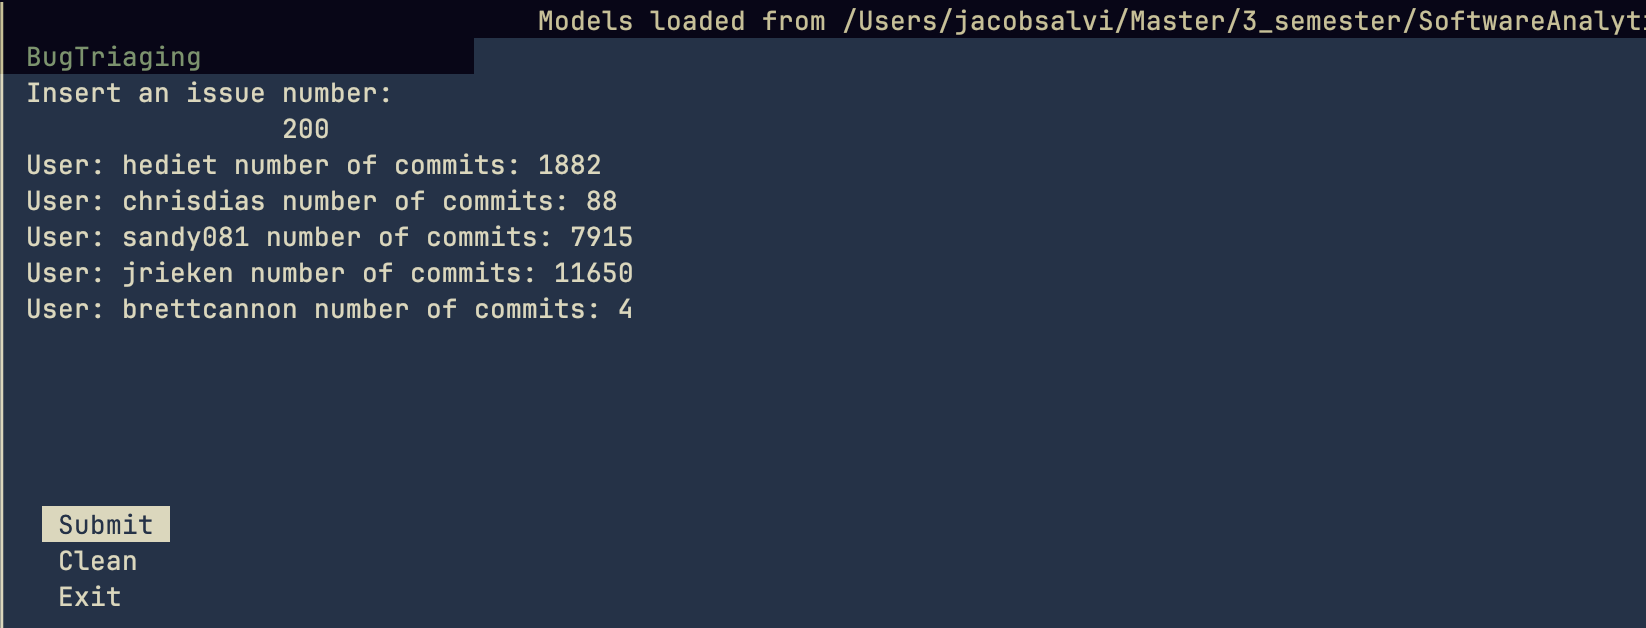
\includegraphics[width=\textwidth]{./tui.png}

To run it is sufficient to run the following code, given that the python environment is set up as described in the README.
\begin{minted}{bash}
python3 src/tui/tui.py
\end{minted}

\section*{Conclusion}
In the project we had the chance of developing a tool for automated bug triaging leveraging using machine learning.\\
Developing this tool we came to appreciated both the strength of such an approach to solve this kind of problem and the challenges in developing it.\\
We also appreciated doing this kind of work in a quite realistic context, given that the vscode repository was used, and can picture many practical application of similar techniques to solve similar challenges in industry.\\
It is also our opinion that we achieved satisfactory results in terms of accuracy.



\end{document}
